% 第三章 系统设计与实现
\chapter{系统设计与实现}

\section{系统概要设计}

\subsection{系统功能模块划分}

本系统面向高校及周边用户群体，以解决即时餐饮决策问题为核心目标，整体划分为四个一级功能模块：用户端小程序、后端 API 服务、智能推荐引擎与数据持久化存储。

\textbf{用户端小程序}运行于微信原生容器中，承担界面渲染、本地状态管理与网络通信职责。其核心功能包括用户身份接入（登录与注册）、静态画像维护（年龄、性别、健康目标、饮食禁忌等）、即时问答交互（用餐时段、预算、口味强度、特殊状态等场景信息采集）、推荐结果浏览与确认、历史记录回看以及菜品与店铺信息的录入。小程序通过微信原生 API 获取用户地理位置，经 HTTPS 协议以 JSON 格式与后端进行加密通信。表现层不处理复杂业务逻辑，仅负责数据采集、本地缓存与结果展示。

\textbf{后端 API 服务}基于 FastAPI 框架构建，作为接口层与业务层的统一载体。接口层承担请求路由、参数校验、身份认证与协议转换职责，通过 Pydantic 模型对请求数据进行自动校验，通过依赖注入机制统一处理 JWT 令牌校验与数据库会话管理，对外暴露标准化 RESTful 端点，对内将合法请求转发至业务层。业务层按照功能域划分为认证服务、画像服务、菜品服务、推荐服务与日志服务：认证服务完成用户注册、登录与令牌管理；画像服务维护用户长期静态特征；菜品服务处理店铺与菜品的增删改查，并在菜品录入后触发语义向量生成流程；推荐服务执行"硬性过滤---向量召回---综合重排"的三阶段推荐流水线；日志服务记录用户选择行为与交互反馈，形成数据闭环。

\textbf{智能推荐引擎}嵌入于业务层之中，是系统的计算核心。其功能涵盖用户目标向量构建、菜品语义向量生成、余弦相似度召回、多目标综合排序及特殊状态加权。引擎通过融合用户静态画像与即时问答结果生成目标向量，基于 sentence-transformers 本地模型完成文本到稠密向量的编码，最终输出兼顾语义相关性、地理可达性与推荐多样性的排序结果。

\textbf{数据持久化存储}对应数据层，采用 MySQL 关系型数据库，通过 SQLAlchemy ORM 进行对象关系映射，持久化存储用户基础信息、用户画像、店铺与菜品数据、历史选择记录及交互日志。数据层通过 InnoDB 存储引擎提供事务支持与行级锁机制，保证并发场景下的数据一致性。

\subsection{系统整体业务流程}

用户从进入系统到完成一次餐饮决策的完整业务流程如下：用户首次使用时通过注册页面提交用户名与密码，后端使用 bcrypt 算法进行加盐哈希后存入用户表，注册成功后返回登录页面；用户登录通过后，后端签发 JWT 令牌，前端将其持久化存储于本地缓存。登录后用户进入个人中心完善静态画像，包括基础生理信息、健康目标、饮食禁忌与口味偏好等。

完成画像后，用户在首页点击"看看今天吃什么"进入问答流程。问答页从后端动态加载题库，以分步式交互引导用户回答用餐时段、预算区间、就餐人数、口味偏好、特殊状态等问题，同时前端通过 \texttt{wx.getLocation} 获取当前经纬度。问答完成后，前端对必填项与定位权限进行基础校验，校验通过后将答案与地理位置打包发送至后端推荐接口。

后端收到请求后，首先读取用户静态画像，结合即时问答结果构建用户目标向量；随后执行硬性过滤，根据预算区间、审核状态与饮食禁忌剔除不可执行候选；对剩余候选计算用户向量与菜品向量的余弦相似度，并融合距离惩罚项与历史平滑项进行综合排序，生成 Top-20 推荐列表及唯一批次 ID；同时将曝光行为写入交互日志。前端以流式卡片形式展示推荐结果，用户浏览后选择最终菜品并发送确认请求。后端将选择结果写入历史记录表，并将确认行为与未选负样本写入交互日志，完成一次完整的推荐闭环。用户后续可在历史页面回看过往选择记录。

\section{数据库设计}

\subsection{概念结构设计}

根据系统功能需求，核心实体包括用户（User）、用户画像（UserProfile）、店铺（Shop）、菜品（Dish）、历史记录（HistoryRecord）、交互日志（InteractionLog）与角色（Role）。各实体间的关联关系如下：用户与用户画像为一对一关系，每个用户有且仅有一份静态画像，通过用户 ID 建立唯一关联；角色与用户为一对多关系，一个角色可包含多个用户，用户通过外键关联至所属角色；店铺与菜品为一对多关系，一家店铺可包含多个菜品，菜品通过外键关联至所属店铺；用户与历史记录为一对多关系，一个用户可产生多条历史选择记录；历史记录与交互日志通过推荐批次 ID 进行逻辑关联，同一批次内的曝光、点击、确认与负样本行为共享相同的批次标识。

\subsection{逻辑结构设计}

在概念模型基础上，将实体及其属性映射为关系数据库中的逻辑表结构，共设计七张核心数据表：用户表、用户画像表、店铺表、菜品表、历史记录表、交互日志表与角色表。

\textbf{用户表（users）}存储用户的基础身份与账号状态信息。该表以自增整数 \texttt{id} 作为主键，\texttt{username} 字段建立唯一索引用于登录检索，\texttt{password\_hash} 字段存储 bcrypt 加盐哈希后的密码密文，\texttt{registration\_time} 记录注册时间戳，\texttt{account\_status} 以布尔值标识账号正常或封禁状态，\texttt{role\_id} 区分普通用户与管理员角色。

\textbf{用户画像表（user\_profiles）}存储用户的长期静态特征。该表以自增整数 \texttt{id} 作为主键，通过 \texttt{user\_id} 外键与用户表建立一对一关联，并建立唯一约束确保一个用户仅对应一份画像。字段涵盖年龄、性别、身高、体重等基础生理信息，活动系数、健康目标等健康相关信息，以及饮食限制、口味偏好、菜系偏好、忌口食材等以字符串或 JSON 格式存储的偏好信息。\texttt{created\_at} 与 \texttt{updated\_at} 分别记录画像的创建与更新时间。

\textbf{店铺表（shops）}存储商户的基础地理与状态信息。主键为自增整数 \texttt{id}，字段包括店铺名称、详细地址、所属城市、经纬度坐标及审批状态。审批状态用于控制店铺及其下属菜品是否可进入推荐候选池。

\textbf{菜品表（dishes）}存储菜品的属性、语义向量与审核信息。主键为自增整数 \texttt{id}，通过 \texttt{shop\_id} 外键关联店铺表。字段包括菜品名称、价格、菜系类型、口味标签、描述文本、主要食材、营养信息及预计算的 768 维语义向量。\texttt{approval\_status} 字段标识审核状态，仅通过审核的菜品可被推荐系统召回。

{\sloppy\textbf{交互日志表（interaction\_logs）}存储推荐过程中的全量交互行为，用于后续的数据分析与模型优化。主键为自增整数 {\ttfamily id}，通过 {\ttfamily user\_id} 关联用户。{\ttfamily recommendation\allowbreak\_batch\allowbreak\_id} 标识推荐批次，{\ttfamily recommended\allowbreak\_dish\allowbreak\_ids} 以 JSON 数组记录曝光列表，{\ttfamily clicked\allowbreak\_dish\allowbreak\_id} 记录用户点击或确认的菜品，{\ttfamily interaction\allowbreak\_type} 以枚举值区分曝光、点击、确认与负样本四类行为。}

{\sloppy\textbf{历史记录表（history\_records）}存储用户的最终选择行为。主键为自增整数 {\ttfamily id}，通过 {\ttfamily user\_id} 与 {\ttfamily dish\_id} 分别关联用户表与菜品表。{\ttfamily recommendation\allowbreak\_batch\allowbreak\_id} 记录本次选择所属的推荐批次，{\ttfamily questionnaire\allowbreak\_snapshot} 以 JSON 格式保存提交问答时的完整场景快照，{\ttfamily is\allowbreak\_first\allowbreak\_recommendation} 标识用户是否采纳了系统首条推荐。}

\textbf{角色表（roles）}存储系统的角色定义，用于实现基于角色的权限控制。主键为自增整数 \texttt{id}，\texttt{name} 字段以唯一约束存储角色名称。用户表通过 \texttt{role\_id} 外键与角色表建立多对一关联，不同角色（如普通用户、管理员）对应不同的系统操作权限。该表使得权限管理从用户表中解耦，便于后续扩展角色类型。

各表的结构化定义如表~\ref{tab:users}至表~\ref{tab:roles}所示。

\begin{table}[htbp]
\centering
\caption{用户表（users）}
\label{tab:users}
\small
\resizebox{\textwidth}{!}{%
\begin{tabular}{>{\bfseries}l >{\ttfamily}l >{\ttfamily}l p{4.5cm}}
\toprule
\textbf{字段名} & \textbf{数据类型} & \textbf{约束} & \textbf{说明} \\
\midrule
id & INT & PRIMARY KEY, AUTO\_INCREMENT & 用户唯一标识 \\
username & VARCHAR(50) & UNIQUE, NOT NULL & 用户名 \\
password\_hash & VARCHAR(255) & NOT NULL & 加盐哈希密码 \\
registration\_time & DATETIME & DEFAULT CURRENT\_TIMESTAMP & 注册时间 \\
account\_status & TINYINT & DEFAULT 1 & 账号状态（1正常，0封禁） \\
role\_id & TINYINT & DEFAULT 1 & 角色ID（1用户，2管理员） \\
\bottomrule
\end{tabular}%
}
\end{table}

\begin{table}[htbp]
\centering
\caption{用户画像表（user\_profiles）}
\label{tab:profiles}
\small
\resizebox{\textwidth}{!}{%
\begin{tabular}{>{\bfseries}l >{\ttfamily}l >{\ttfamily}l p{4.5cm}}
\toprule
\textbf{字段名} & \textbf{数据类型} & \textbf{约束} & \textbf{说明} \\
\midrule
id & INT & PRIMARY KEY, AUTO\_INCREMENT & 画像唯一标识 \\
user\_id & INT & FOREIGN KEY, UNIQUE & 关联用户ID \\
age & INT & --- & 年龄 \\
gender & TINYINT & --- & 性别（0女，1男，2保密） \\
height & INT & --- & 身高（cm） \\
weight & INT & --- & 体重（kg） \\
activity\_level & TINYINT & --- & 活动系数（1-5） \\
health\_goal & VARCHAR(100) & --- & 健康目标 \\
dietary\_restrictions & VARCHAR(255) & --- & 饮食限制 \\
taste\_preferences & VARCHAR(255) & --- & 口味偏好 \\
cuisine\_preferences & VARCHAR(255) & --- & 菜系偏好 \\
taboo\_ingredients & VARCHAR(255) & --- & 忌口食材 \\
created\_at & DATETIME & DEFAULT CURRENT\_TIMESTAMP & 创建时间 \\
updated\_at & DATETIME & ON UPDATE CURRENT\_TIMESTAMP & 更新时间 \\
\bottomrule
\end{tabular}%
}
\end{table}

\begin{table}[htbp]
\centering
\caption{店铺表（shops）}
\label{tab:shops}
\small
\resizebox{\textwidth}{!}{%
\begin{tabular}{>{\bfseries}l >{\ttfamily}l >{\ttfamily}l p{4.5cm}}
\toprule
\textbf{字段名} & \textbf{数据类型} & \textbf{约束} & \textbf{说明} \\
\midrule
id & INT & PRIMARY KEY, AUTO\_INCREMENT & 店铺唯一标识 \\
name & VARCHAR(100) & NOT NULL & 店铺名称 \\
address & VARCHAR(255) & --- & 详细地址 \\
city & VARCHAR(50) & --- & 所属城市 \\
latitude & DECIMAL(10,8) & --- & 纬度 \\
longitude & DECIMAL(11,8) & --- & 经度 \\
approval\_status & TINYINT & DEFAULT 0 & 审批状态（0待审，1通过） \\
created\_at & DATETIME & DEFAULT CURRENT\_TIMESTAMP & 创建时间 \\
\bottomrule
\end{tabular}%
}
\end{table}

\begin{table}[htbp]
\centering
\caption{菜品表（dishes）}
\label{tab:dishes}
\small
\resizebox{\textwidth}{!}{%
\begin{tabular}{>{\bfseries}l >{\ttfamily}l >{\ttfamily}l p{4.5cm}}
\toprule
\textbf{字段名} & \textbf{数据类型} & \textbf{约束} & \textbf{说明} \\
\midrule
id & INT & PRIMARY KEY, AUTO\_INCREMENT & 菜品唯一标识 \\
shop\_id & INT & FOREIGN KEY, NOT NULL & 关联店铺ID \\
name & VARCHAR(100) & NOT NULL & 菜品名称 \\
price & DECIMAL(10,2) & NOT NULL & 价格（元） \\
cuisine\_type & VARCHAR(50) & --- & 菜系类型 \\
taste\_tags & VARCHAR(255) & --- & 口味标签（JSON数组） \\
description & TEXT & --- & 菜品描述 \\
ingredients & VARCHAR(255) & --- & 主要食材 \\
nutrition\_info & VARCHAR(255) & --- & 营养信息（JSON） \\
vector & JSON & --- & 语义向量（768维数组） \\
approval\_status & TINYINT & DEFAULT 0 & 审批状态 \\
created\_at & DATETIME & DEFAULT CURRENT\_TIMESTAMP & 创建时间 \\
\bottomrule
\end{tabular}%
}
\end{table}

\begin{table}[htbp]
\centering
\caption{历史记录表（history\_records）}
\label{tab:history}
\small
\resizebox{\textwidth}{!}{%
\begin{tabular}{>{\bfseries}l >{\ttfamily}l >{\ttfamily}l p{4.5cm}}
\toprule
\textbf{字段名} & \textbf{数据类型} & \textbf{约束} & \textbf{说明} \\
\midrule
id & INT & PRIMARY KEY, AUTO\_INCREMENT & 记录唯一标识 \\
user\_id & INT & FOREIGN KEY, NOT NULL & 用户ID \\
dish\_id & INT & FOREIGN KEY, NOT NULL & 选择的菜品ID \\
recommendation\_batch\_id & VARCHAR(64) & NOT NULL & 推荐批次ID \\
questionnaire\_snapshot & JSON & --- & 问答快照 \\
is\_first\_recommendation & TINYINT & DEFAULT 1 & 是否采纳首条推荐 \\
created\_at & DATETIME & DEFAULT CURRENT\_TIMESTAMP & 创建时间 \\
\bottomrule
\end{tabular}%
}
\end{table}

\begin{table}[htbp]
\centering
\caption{交互日志表（interaction\_logs）}
\label{tab:logs}
\small
\resizebox{\textwidth}{!}{%
\begin{tabular}{>{\bfseries}l >{\ttfamily}l >{\ttfamily}l p{4.5cm}}
\toprule
\textbf{字段名} & \textbf{数据类型} & \textbf{约束} & \textbf{说明} \\
\midrule
id & INT & PRIMARY KEY, AUTO\_INCREMENT & 日志唯一标识 \\
user\_id & INT & FOREIGN KEY, NOT NULL & 用户ID \\
recommendation\_batch\_id & VARCHAR(64) & NOT NULL & 推荐批次ID \\
recommended\_dish\_ids & JSON & --- & 推荐列表（菜品ID数组） \\
clicked\_dish\_id & INT & --- & 点击/确认的菜品ID \\
interaction\_type & TINYINT & NOT NULL & 交互类型（1曝光，2点击，3确认，4负样本） \\
interaction\_time & DATETIME & DEFAULT CURRENT\_TIMESTAMP & 交互时间 \\
\bottomrule
\end{tabular}%
}
\end{table}

\begin{table}[htbp]
\centering
\caption{角色表（roles）}
\label{tab:roles}
\small
\resizebox{\textwidth}{!}{%
\begin{tabular}{>{\bfseries}l >{\ttfamily}l >{\ttfamily}l p{4.5cm}}
\toprule
\textbf{字段名} & \textbf{数据类型} & \textbf{约束} & \textbf{说明} \\
\midrule
id & INT & PRIMARY KEY, AUTO\_INCREMENT & 角色唯一标识 \\
name & VARCHAR(50) & UNIQUE, NOT NULL & 角色名称（如"管理员"） \\
\bottomrule
\end{tabular}%
}
\end{table}

\section{系统详细设计}

\subsection{前端交互详细设计}

前端基于微信小程序原生框架，采用多页面架构组织功能。核心页面包括登录/注册页、首页、问答页、推荐页、历史页、个人中心页、画像编辑页及菜品录入页。各页面之间通过路由跳转与事件回调进行协作，本地状态通过 Page 对象的 data 属性进行管理，全局状态（如用户令牌、基础信息）通过 App 实例的 globalData 共享。

首页作为系统入口，承担导航与状态展示职责。页面顶部展示用户头像、昵称及当前定位地址；中部以卡片形式提供"看看今天吃什么"与"浏览附近美食"两个核心入口。定位功能通过 \texttt{wx.getLocation} 获取经纬度，经逆地理编码转换为可读地址。若用户拒绝授权，页面显示提示信息并引导手动选择城市，避免无意义的后续请求。

问答页采用分步式交互设计，以降低用户的认知负荷。页面从后端动态加载题库，每屏展示一至两道题目，底部配置进度指示器。题目类型涵盖单选、多选、滑条与文本输入四种，通过条件渲染适配不同题型的交互组件。答题过程中，已填写的答案保存在页面状态对象中，若用户意外退出后返回，可从本地缓存恢复作答进度，保证交互连续性。问答完成后，前端对必填项与定位权限进行基础校验，校验通过后将答案与地理位置打包发送至推荐接口。

推荐页采用流式列表布局展示候选菜品。每条推荐以卡片形式呈现，包含菜品图片、名称、价格、店铺名、直线距离与综合得分。页面顶部展示当前场景摘要（如"晚餐 · 50-100元 · 清淡"），帮助用户确认系统已正确理解其需求。用户点击卡片进入详情页，可查看菜品描述、食材、营养成分及店铺信息；详情页底部提供"就决定是你了"确认按钮，点击后发送确认请求并展示成功反馈。

历史页按时间倒序展示用户过往选择记录，支持点击查看详情与重新推荐。个人中心页展示用户基础信息与画像摘要，提供进入画像编辑与菜品录入的入口。画像编辑页采用表单布局，支持对静态画像字段的增量修改。菜品录入页面向管理员或授权用户，提供店铺与菜品信息的表单提交，提交成功后触发后端向量化流程。

\subsection{认证模块详细设计}

认证模块是系统的安全入口，负责用户身份的注册、校验与会话管理。模块的核心流程分为注册、登录与令牌校验三个环节。

在注册环节，前端采集用户名与密码后发送至后端。后端首先查询用户表验证用户名是否已存在，若存在则返回业务错误；若不存在，则使用 bcrypt 算法对明文密码进行加盐哈希，生成不可逆的密码摘要后存入用户表，返回用户基础信息。bcrypt 算法通过可配置的工作因子（work factor）增加哈希计算耗时，有效抵抗彩虹表攻击与暴力破解。

在登录环节，后端根据用户名查询用户记录，使用 bcrypt 的校验函数比对明文密码与存储的哈希值。若校验通过且账号状态正常，则使用 \texttt{python-jose} 库签发 JWT 访问令牌。令牌 Payload 包含用户唯一标识与用户名，并设置 24 小时的有效期。后端将令牌返回给前端，前端将其存入本地缓存，用于后续请求的认证。

在令牌校验环节，受保护接口通过依赖注入机制统一处理认证逻辑。后端从请求头的 \texttt{Authorization} 字段中提取 Bearer 令牌，验证签名与过期时间，并查询数据库确认用户存在且未被禁。任一校验失败均返回对应的 HTTP 状态码（401 未认证或 403 无权限），拦截非法请求。

\subsection{画像模块详细设计}

画像模块负责用户静态画像的生命周期管理，包括创建、查询与更新。静态画像是推荐系统个性化基础，包含用户的长期稳定特征。

用户首次登录后进入画像编辑页面，前端将年龄、性别、身高、体重、活动系数、健康目标、饮食禁忌、口味偏好、菜系偏好及忌口食材等字段打包发送至后端。后端检查该用户是否已存在画像记录，若不存在则创建新记录，若存在则返回冲突错误。画像创建成功后，用户可随时进入编辑页修改信息。

在更新环节，模块采用部分更新策略。前端仅提交用户修改的字段，后端通过 Pydantic 模型的 \texttt{exclude\_unset=True} 参数过滤未传入的字段，仅对显式指定的属性执行赋值操作，其余字段保持原值不变。这一设计避免了用户在编辑少量信息时需要重复填写全部内容的问题，显著提升了交互效率。更新完成后，后端提交事务并返回更新后的画像数据。

\subsection{菜品与向量化模块详细设计}

菜品模块负责店铺与菜品信息的录入、查询与管理，并向量化模块在菜品录入后触发语义向量生成流程，为推荐系统的语义召回提供数据基础。

菜品向量构建采用文本拼接策略。系统将菜品的名称、菜系类型、口味标签、描述文本、主要食材及所属城市等结构化字段按固定模板拼接为一段连贯的语义文本。例如，一道"麻婆豆腐"生成的语义文本为："菜品名称：麻婆豆腐，菜系：川菜，口味：麻辣、鲜香、重口味，描述：经典川菜，豆腐嫩滑，麻辣鲜香，下饭神器，食材：豆腐、牛肉末、豆瓣酱、花椒、辣椒，城市：杭州"。该文本通过 sentence-transformers 本地模型编码为 768 维稠密向量，经 L2 归一化后存储于菜品表的 \texttt{vector} 字段。

向量化流程在菜品录入时同步触发。后端接收菜品信息并持久化后，调用向量生成服务。服务首先检查模型可用性，若模型未加载成功则返回 503 错误，拒绝写入无效向量；若模型可用，则执行编码并将向量回写至数据库。整个流程在数据库事务中完成，确保菜品记录与向量数据的一致性。

\subsection{历史与日志模块详细设计}

历史与日志模块负责推荐结果的持久化存储与交互行为的闭环记录，为后续的数据分析与模型优化提供原始数据。

历史记录模块在用户确认选择后触发。后端接收批次 ID 与菜品 ID，查询该批次对应的曝光日志以验证请求合法性，随后将用户 ID、菜品 ID、批次 ID 及问答快照写入历史记录表。若用户选择的是推荐列表的首条菜品，\texttt{is\_first\_recommendation} 标记为真，便于后续评估推荐准确率。

交互日志模块记录推荐全链路中的关键行为节点。在推荐阶段，系统将批次 ID、用户 ID 与 Top-20 推荐列表以曝光类型写入日志；在用户浏览阶段，前端异步上报点击行为；在确认阶段，后端将确认行为写入日志，并将推荐列表中未被选择的菜品作为负样本逐一写入日志。通过同一批次 ID 关联曝光、点击、确认与负样本记录，形成完整的交互闭环。

\subsection{推荐模块详细设计}

推荐引擎是系统的计算核心，采用"硬性过滤---向量召回---综合重排"的三阶段流水线架构。该设计在保证约束可执行性的前提下，通过语义向量捕捉用户即时意图，并通过多目标融合实现排序优化。

\textbf{（1）双通道用户向量建模}

用户目标向量的构建融合静态画像与即时问答两个通道。静态画像通道将用户的健康目标、口味偏好、菜系偏好与忌口食材拼接为基础偏好文本；即时问答通道将用餐时段、预算区间、就餐人数、六维口味强度（辣/麻/酸/甜/咸/油）及特殊状态拼接为场景文本。两段文本分别经 sentence-transformers 编码为 768 维向量 $V_{base}$ 与 $V_{scene}$，按 0.4 与 0.6 的权重加权融合：

\begin{equation}
V_{fusion} = 0.4 \cdot V_{base} + 0.6 \cdot V_{scene}
\end{equation}

融合后的向量经 L2 归一化得到用户目标向量 $V_u$：

\begin{equation}
V_u = \frac{V_{fusion}}{\|V_{fusion}\|_2}
\end{equation}

权重分配的依据在于：静态画像反映长期稳定偏好，但无法捕捉当日波动；即时问答直接表征当前决策场景，但缺乏个性化基础。0.6 的问答权重确保了推荐结果对当前场景的敏感性。

\textbf{（2）菜品向量构建}

菜品向量采用结构化文本拼接策略。设菜品 $d$ 具有名称 $n_d$、菜系 $c_d$、口味标签 $t_d$、描述 $desc_d$、食材 $ing_d$ 与城市 $city_d$ 等属性，则语义文本 $T_d$ 的生成模板为：

\begin{equation}
\begin{aligned}
T_d = {} & \text{``菜品名称：''} n_d \text{``，菜系：''} c_d \text{``，口味：''} t_d \\
       & \text{``，描述：''} desc_d \text{``，食材：''} ing_d \text{``，城市：''} city_d
\end{aligned}
\end{equation}

该文本经编码器 $Encoder(\cdot)$ 映射为向量 $V_d$，并执行 L2 归一化：

\begin{equation}
V_d = \frac{Encoder(T_d)}{\|Encoder(T_d)\|_2}
\end{equation}

\textbf{（3）硬性过滤设计}

硬性过滤阶段通过数据库查询快速缩小候选空间。过滤条件包括：
\begin{itemize}[leftmargin=2em, itemsep=0.2em]
    \item 预算约束：将用户选择的预算区间映射为价格上下限 $[p_{min}, p_{max}]$，仅保留价格落在区间内的菜品；
    \item 审核约束：仅保留 \texttt{approval\_status = 1} 的已审核菜品；
    \item 禁忌约束：解析用户画像中的忌口食材列表 $Taboo = \{t_1, t_2, ..., t_m\}$，剔除食材字段包含任一忌口关键词的菜品。
\end{itemize}

若过滤后候选集 $D_c = \emptyset$，系统终止后续计算并返回提示信息。

\textbf{（4）向量召回设计}

在候选集 $D_c$ 上，计算用户目标向量 $V_u$ 与每个候选菜品向量 $V_d$ 的余弦相似度。由于双方均已 L2 归一化，余弦相似度可简化为向量点积：

\begin{equation}
Sim(V_u, V_d) = \frac{V_u \cdot V_d}{\|V_u\| \|V_d\|} = V_u \cdot V_d
\end{equation}

该设计的计算复杂度为 $O(|D_c| \cdot dim)$，其中 $dim = 768$ 为向量维度。在候选规模可控的前提下（通常 50--300），该计算可在毫秒级完成。

\textbf{（5）综合重排设计}

综合重排在语义相似度基础上引入地理可达性与推荐多样性因素。

距离惩罚项建模用户位置与店铺位置之间的空间衰减关系。设用户当前位置为 $loc_u = (lat_u, lon_u)$，菜品所属店铺位置为 $loc_d = (lat_d, lon_d)$，两者之间的直线距离为 $dist(u, d)$（单位：公里），最大有效距离 $D_{max} = 10$ 公里。距离惩罚项定义为：

\begin{equation}
DistPenalty(d) = \max\left(0, 1 - \frac{dist(u, d)}{D_{max}}\right)
\end{equation}

当距离为 0 时惩罚项取最大值 1；当距离超过 10 公里时惩罚项归零，避免推荐不可达候选。

历史平滑项用于防止同一菜品被反复推荐，增加结果多样性。设 $count_{recent}(d)$ 为菜品 $d$ 在最近 7 天内被推荐至该用户的次数，衰减系数 $\lambda = 0.3$，最小平滑值 $\epsilon = 0.1$。历史平滑项定义为：

\begin{equation}
HistorySmooth(d) = \max\left(\epsilon, 1 - \lambda \cdot count_{recent}(d)\right)
\end{equation}

特殊状态加权项根据用户选择的特殊状态对符合条件的菜品施加增益。系统维护状态-标签映射规则，例如"正在减脂"状态对带有"清淡""低热量""蒸""煮"标签的菜品施加 1.3 倍增益；"胃不舒服"状态对带有"粥""汤""蒸"标签的菜品施加 1.4 倍增益。设状态对应的加权系数为 $Bonus(d) \in [1.0, 1.4]$。

最终综合得分 $S_{final}$ 的计算公式为：

\begin{equation}
S_{final} = \left(\alpha \cdot Sim(V_u, V_d) + \beta \cdot DistPenalty(d) + \gamma \cdot HistorySmooth(d)\right) \cdot Bonus(d)
\end{equation}

其中权重系数满足 $\alpha + \beta + \gamma = 1$，具体取值为 $\alpha = 0.6$（语义相关性）、$\beta = 0.3$（地理可达性）、$\gamma = 0.1$（多样性）。系统按 $S_{final}$ 降序排列，取 Top-20 作为最终推荐列表。

\textbf{（6）算法复杂度分析}

设硬性过滤后的候选规模为 $k$，向量维度为 $d = 768$。硬性过滤依托数据库索引，时间复杂度为 $O(\log n + k)$；向量召回阶段计算 $k$ 个点积，复杂度为 $O(k \cdot d)$；综合重排阶段计算距离、历史平滑与特殊状态加权，复杂度为 $O(k)$；最终排序采用快速排序，复杂度为 $O(k \log k)$。总体时间复杂度为：

\begin{equation}
O(k \cdot d + k \log k)
\end{equation}

在工程实践中，$k$ 通常控制在 300 以内，因此向量计算为主要性能瓶颈。该复杂度在单线程环境下可在 1 秒内完成，满足实时性要求。

\textbf{（7）推荐算法伪代码}

\begin{lstlisting}[language=Python, caption={基于画像与问答的餐饮推荐算法}, label={lst:algo}]
算法：基于画像与问答的餐饮推荐算法
输入：用户画像 profile，问答结果 answers，用户位置 (lat, lon)
输出：Top-K 推荐列表 R

1.  解析预算区间 [p_min, p_max] <- BudgetMap(answers.budget)
2.  候选过滤：
    D_c <- {d in Dishes | d.price in [p_min, p_max] 
           and d.approval_status = 1
           and d.ingredients intersect profile.taboo_ingredients = empty}
3.  若 D_c = empty：返回提示"当前条件下无符合条件的菜品"
4.  构建用户目标向量：
    V_u <- Normalize(0.4*Encode(BaseText(profile)) + 0.6*Encode(SceneText(answers)))
5.  对每个候选菜品 d in D_c：
6.      Sim(d) <- DotProduct(V_u, d.vector)
7.      DistPenalty(d) <- max(0, 1 - Haversine((lat,lon), d.location) / 10)
8.      HistorySmooth(d) <- max(0.1, 1 - 0.3 * RecentCount(d, 7days))
9.      Bonus(d) <- SpecialStateBonus(answers.special_state, d.taste_tags)
10.     Score(d) <- (0.6*Sim(d) + 0.3*DistPenalty(d) + 0.1*HistorySmooth(d)) * Bonus(d)
11. 按 Score(d) 降序排序
12. R <- Top-20(D_c)
13. batch_id <- GenerateUUID()
14. 写入交互日志：ExposureLog(batch_id, user_id, R)
15. 返回 (batch_id, R)
\end{lstlisting}

\section{系统实现}

\subsection{认证与鉴权模块实现}

认证与鉴权模块实现用户身份的注册、登录与会话管理。后端基于 FastAPI 提供注册、登录两个核心端点，并通过依赖注入机制为受保护接口提供统一的 JWT 校验入口。注册时采用 bcrypt 自适应哈希生成密码摘要；登录时校验密码与账号状态后签发 JWT 令牌，令牌有效期设置为 24 小时。

\begin{lstlisting}[language=Python, caption={认证模块后端核心实现}]
@router.post("/register", response_model=dict)
def register(body: UserRegister, db: Session = Depends(get_db)):
    if db.query(User).filter(User.username == body.username).first():
        raise HTTPException(status_code=400, detail="用户名已存在")
    user = User(
        id=gen_uuid(),
        username=body.username,
        password_hash=hash_password(body.password),
        registration_time=datetime.utcnow(),
    )
    db.add(user)
    db.commit()
    return {"message": "注册成功", "user_id": user.id}

@router.post("/login", response_model=TokenResponse)
def login(body: UserLogin, db: Session = Depends(get_db)):
    user = db.query(User).filter(User.username == body.username).first()
    if not user or not verify_password(body.password, user.password_hash):
        raise HTTPException(status_code=401, detail="用户名或密码错误")
    token = create_access_token(user.id)
    is_admin = user.role.name == "管理员" if user.role else False
    return TokenResponse(access_token=token, username=user.username, is_admin=is_admin)
\end{lstlisting}

前端登录页提供用户名与密码输入框，支持跳转至注册页；注册页采集用户名与密码，提交后自动返回登录页。登录成功后前端将 JWT 令牌持久化存储，用于后续请求的认证头部。

\begin{figure}[H]
\centering
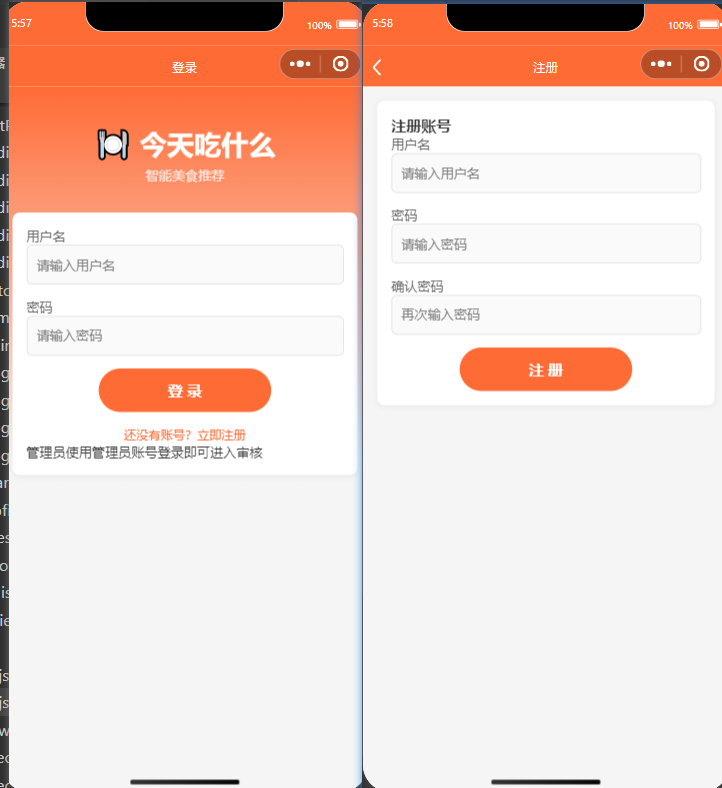
\includegraphics[width=0.8\textwidth,height=0.75\textheight,keepaspectratio]{images/3-1.png}
\caption{登录页与注册页界面截图}
\label{fig:3-1}
\end{figure}

\subsection{用户画像模块实现}

用户画像模块实现静态画像的创建、查询与增量更新。后端采用 Pydantic 的 \texttt{exclude\_unset=True} 特性实现部分更新，仅修改客户端显式传入的字段，避免移动端碎片化编辑场景下的全量表单提交。画像与用户之间通过唯一外键建立严格的一对一关系。

\begin{lstlisting}[language=Python, caption={画像模块后端核心实现}]
@router.get("/", response_model=UserProfileOut)
def get_profile(user: User = Depends(get_current_user), db: Session = Depends(get_db)):
    profile = db.query(UserProfile).filter(UserProfile.user_id == user.id).first()
    if not profile:
        raise HTTPException(status_code=404, detail="尚未创建画像")
    return profile

@router.post("/", response_model=UserProfileOut)
def create_profile(body: UserProfileCreate, user: User = Depends(get_current_user), db: Session = Depends(get_db)):
    existing = db.query(UserProfile).filter(UserProfile.user_id == user.id).first()
    if existing:
        raise HTTPException(status_code=400, detail="画像已存在，请使用PUT更新")
    profile = UserProfile(user_id=user.id, **body.model_dump(exclude_none=True))
    db.add(profile)
    db.commit()
    db.refresh(profile)
    return profile

@router.put("/", response_model=UserProfileOut)
def update_profile(body: UserProfileCreate, user: User = Depends(get_current_user), db: Session = Depends(get_db)):
    profile = db.query(UserProfile).filter(UserProfile.user_id == user.id).first()
    if not profile:
        raise HTTPException(status_code=404, detail="尚未创建画像")
    update_data = body.model_dump(exclude_unset=True)
    for key, val in update_data.items():
        setattr(profile, key, val)
    db.commit()
    db.refresh(profile)
    return profile
\end{lstlisting}

前端画像编辑页采用表单布局，分区块展示基础生理信息、健康目标、饮食限制与口味偏好。用户修改任意字段后点击保存，前端仅将变更字段发送至后端执行增量更新。

\begin{figure}[H]
\centering
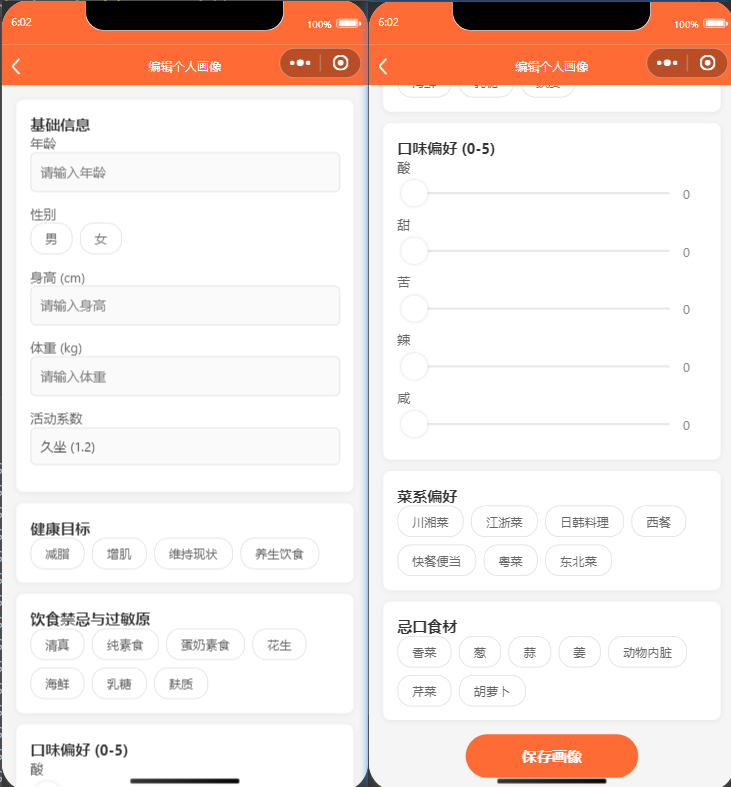
\includegraphics[width=0.8\textwidth,height=0.75\textheight,keepaspectratio]{images/3-2.png}
\caption{画像编辑页界面截图}
\label{fig:3-2}
\end{figure}

\subsection{智能推荐模块实现}

智能推荐模块是系统的核心，实现问答题库管理、三阶段推荐计算与选择确认。后端题库以结构化 JSON 形式存储，支持单选、多选、滑条与文本输入四种题型动态加载。推荐接口执行完整的"硬性过滤---向量召回---综合重排"流水线：首先解析预算区间并执行数据库层面的硬性过滤；随后调用向量服务构建用户目标向量并计算余弦相似度；最后融合距离惩罚、历史平滑与特殊状态加权生成 Top-20 推荐列表及唯一批次 ID。确认接口接收批次 ID 与菜品 ID，将选择结果写入历史记录，并将曝光列表中的未选项作为负样本写入交互日志。

\begin{lstlisting}[language=Python, caption={推荐模块后端核心实现}]
@router.post("/submit", response_model=RecommendationResponse)
def submit_and_recommend(
    answers: QuestionnaireAnswers,
    latitude: float = 0.0,
    longitude: float = 0.0,
    user: User = Depends(get_current_user),
    db: Session = Depends(get_db),
):
    batch_id = gen_uuid()
    # 硬性过滤：预算 + 审核状态
    q = db.query(Dish).filter(Dish.is_approved == True)
    budget_range = BUDGET_RANGE.get(answers.budget, (0, 99999))
    q = q.filter(Dish.price >= budget_range[0], Dish.price <= budget_range[1])
    candidates: List[Dish] = q.all()

    # 向量召回
    user_vector = _build_user_vector(answers, profile)
    candidate_vectors = [np.array(d.vector) for d in candidates if d.vector]
    similarities = cosine_similarity([user_vector], candidate_vectors)[0]
    vector_scores = {candidates[i].id: similarities[i] for i in range(len(candidates))}

    # 综合排序
    scored = []
    for d in candidates:
        sim_score = vector_scores[d.id]
        special_bonus = _special_state_bonus(answers.special_state, d)
        sim_score = sim_score * 0.8 + special_bonus * 0.2
        dist = haversine_km(latitude, longitude, d.latitude or 0, d.longitude or 0)
        dist_penalty = max(0, 1 - dist / 10)
        final = 0.6 * sim_score + 0.3 * dist_penalty + 0.1 * history_score
        scored.append((d, final, dist))
    scored.sort(key=lambda x: x[1], reverse=True)
    top_n = scored[:20]
    # 写入曝光日志
    log = InteractionLog(user_id=user.id, recommendation_batch_id=batch_id,
        recommended_dishes=[d.id for d, _, _ in top_n], ...)
    db.add(log); db.commit()
    return RecommendationResponse(batch_id=batch_id, items=items)

@router.post("/confirm")
def confirm_selection(body: SelectionConfirm, user: User = Depends(get_current_user), db: Session = Depends(get_db)):
    dish = db.query(Dish).filter(Dish.id == body.selected_dish_id).first()
    log = db.query(InteractionLog).filter(
        InteractionLog.recommendation_batch_id == body.batch_id).first()
    is_first = log.recommended_dishes[0] == body.selected_dish_id if log else False
    record = HistoryRecord(user_id=user.id, recommendation_batch_id=body.batch_id,
        selected_dish_id=body.selected_dish_id, dining_time=datetime.utcnow(),
        is_first_recommendation=is_first)
    db.add(record); db.commit()
    return {"message": "选择已记录", "dish_name": dish.name}
\end{lstlisting}

向量生成服务封装 sentence-transformers 模型的加载与编码逻辑，提供菜品向量生成与用户向量融合两个核心函数。模型加载采用 \texttt{local\_files\_only=True} 参数，避免运行时自动联网下载。

\begin{lstlisting}[language=Python, caption={向量生成服务核心实现}]
def vectorize_text(text: str, dim: int = DEFAULT_VECTOR_DIM) -> List[float]:
    model = _sentence_model()
    if model is None:
        raise ModelUnavailableError("sentence-transformers 模型不可用")
    embedding = model.encode([text], normalize_embeddings=True)[0]
    vec = [float(v) for v in embedding.tolist()]
    return [round(float(x), 8) for x in _l2_normalize(vec)]

def generate_dish_vector(name: str, cuisine=None, taste_tags=None,
        description=None, ingredients=None, city=None, ...) -> List[float]:
    taste_scores = infer_taste_scores(name, description, taste_tags, cuisine)
    text = build_dish_text(name=name, cuisine=cuisine, taste_tags=taste_tags,
        description=description, ingredients=ingredients, city=city,
        taste_scores=taste_scores)
    return _local_model_vectorize(text, dim)

def generate_user_vector(taste_preferences, cuisine_preferences,
        avoid_foods, answers, ...) -> List[float]:
    text = "\\n".join([
        f"用户口味偏好:{tastes}",
        f"用户菜系偏好:{cuisines}",
        f"当前时段:{answers.get('meal_time', '')}",
        f"当前场景人数:{answers.get('dining_scene', '')}",
        # ... 更多字段拼接
    ])
    return _local_model_vectorize(text, dim)
\end{lstlisting}

前端问答页采用分步式布局，从后端动态加载题库，每屏展示一至两道题目，底部配置进度指示器。答题过程中答案保存在页面状态中，支持意外退出后的进度恢复。问答完成后前端执行必填项与定位权限的双重校验，通过后将答案与经纬度打包发送。

\begin{figure}[H]
\centering
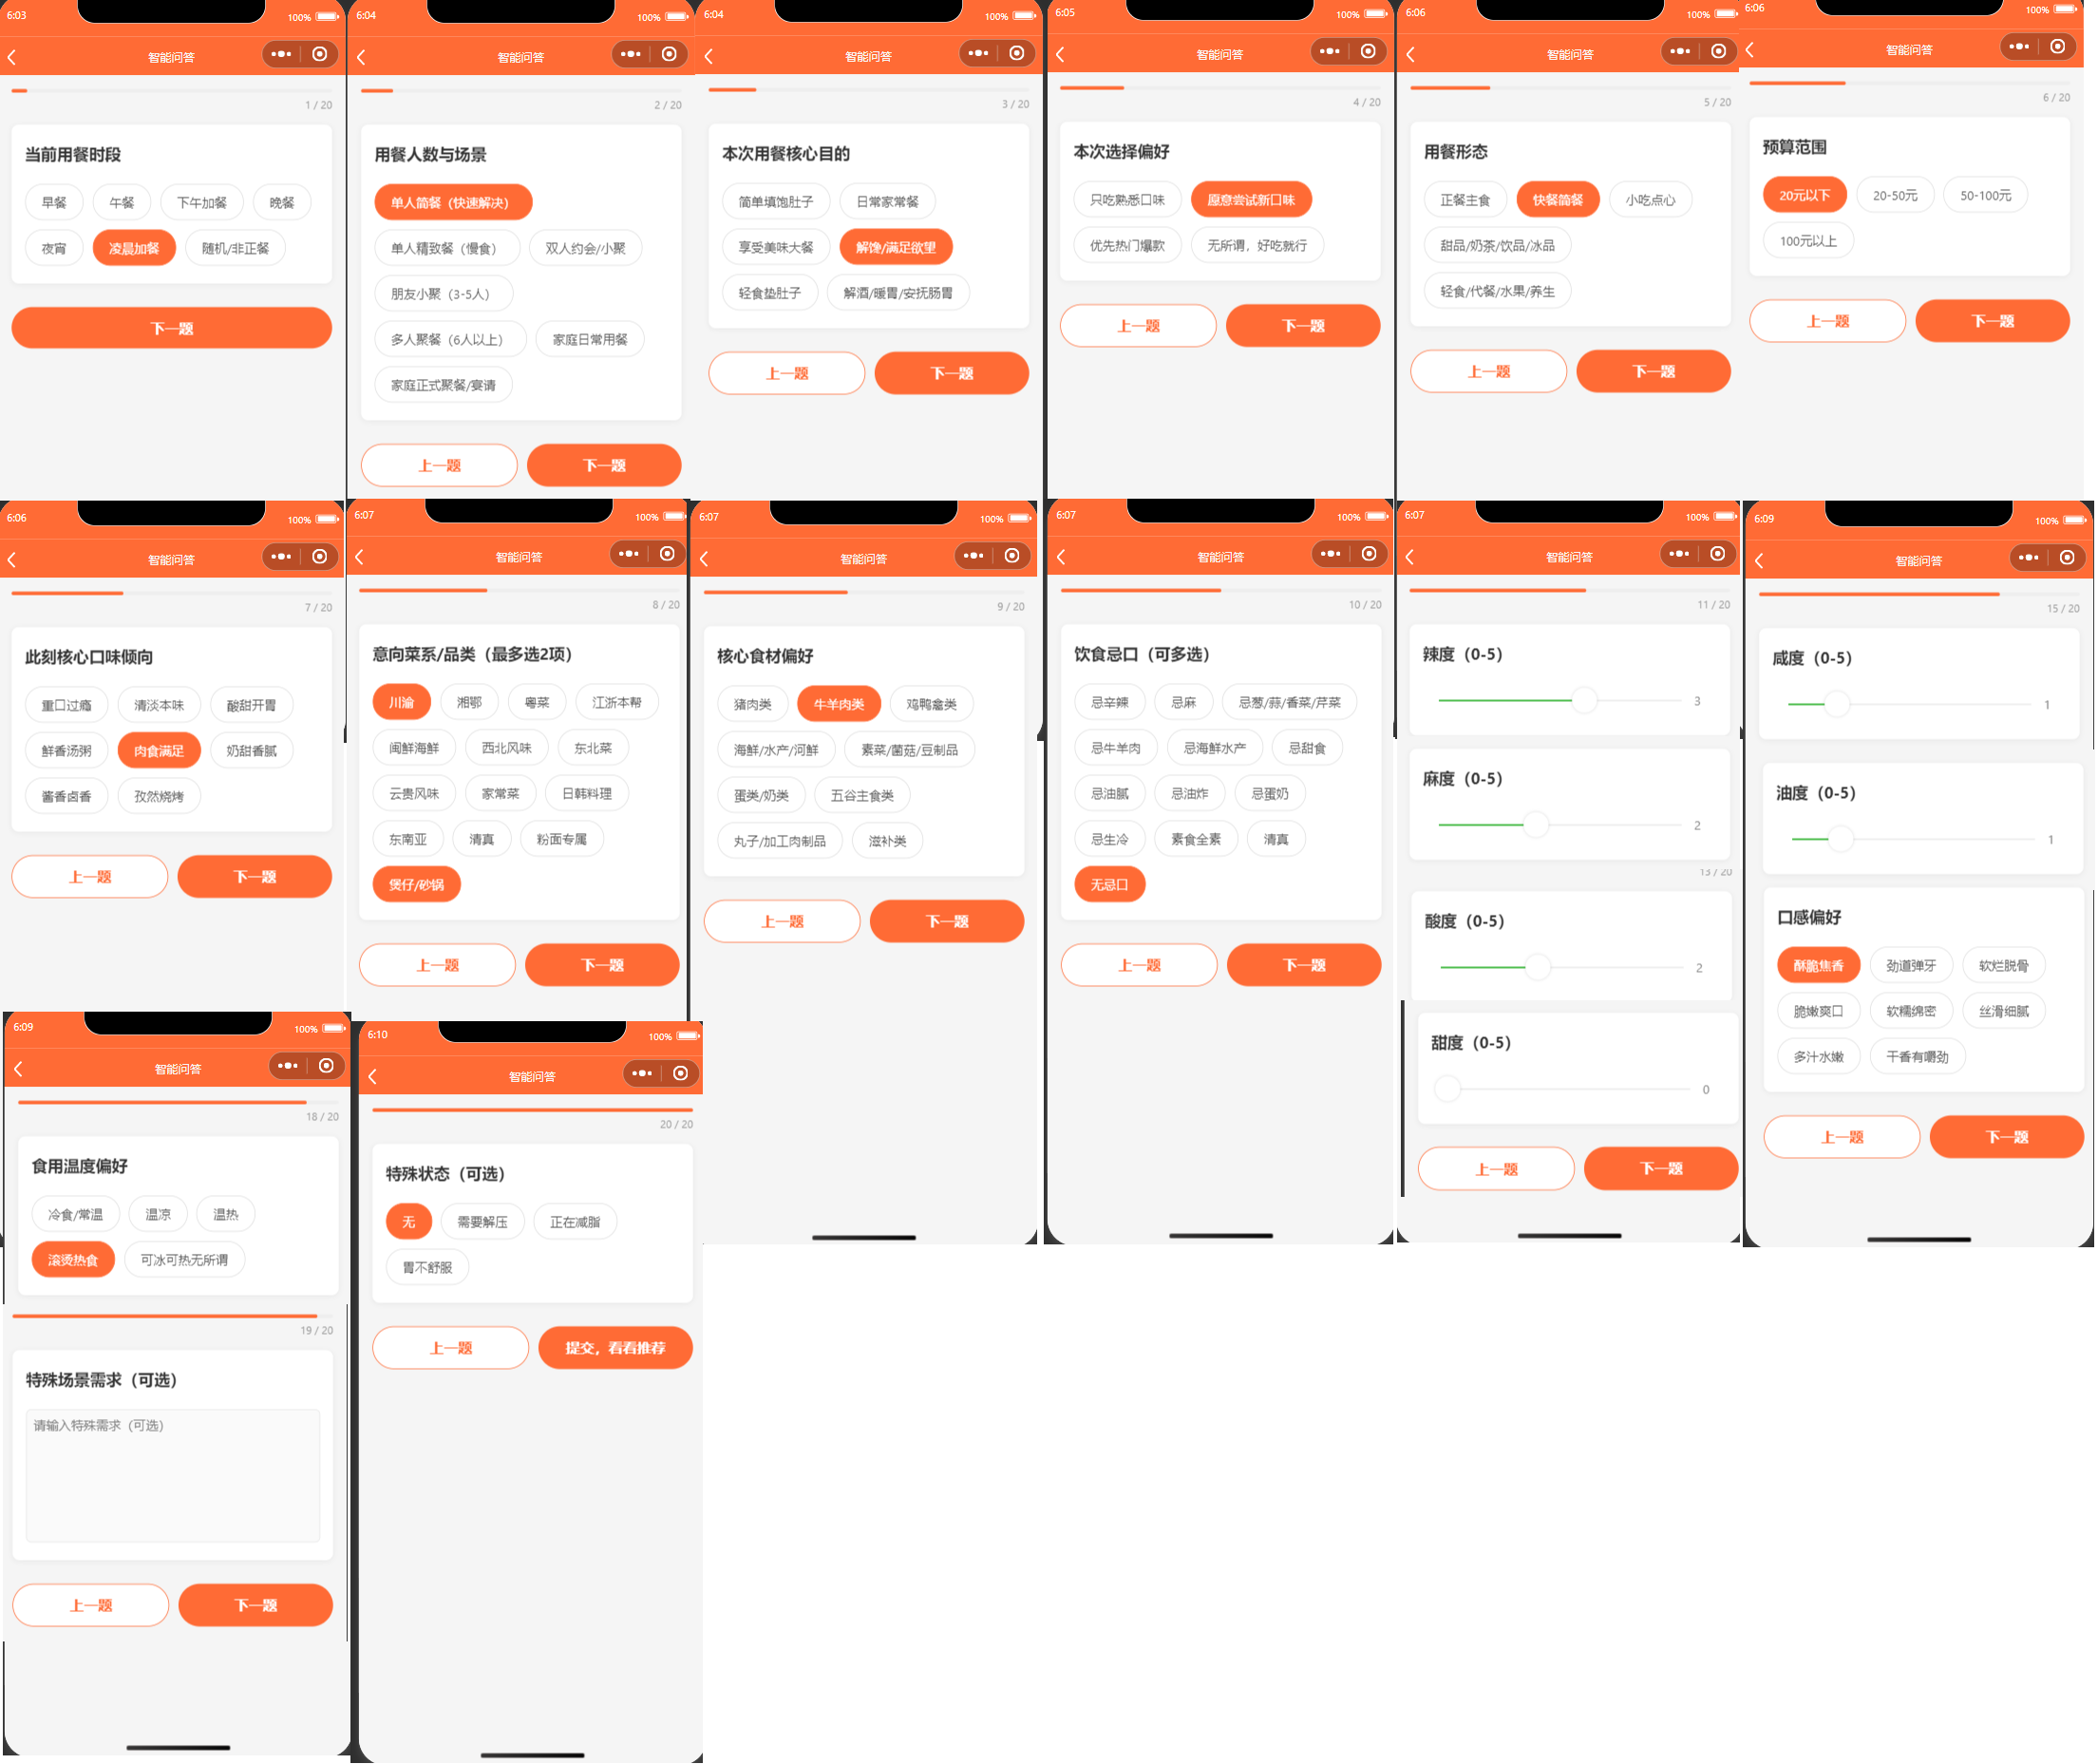
\includegraphics[width=0.8\textwidth]{images/3-3.png}
\caption{问答页面截图}
\label{fig:3-3}
\end{figure}

推荐结果页以卡片流形式展示候选菜品，每张卡片包含菜品图片、名称、价格、店铺名、直线距离与综合得分。页面顶部展示当前场景摘要。用户点击卡片进入详情页，可查看菜品描述、食材与营养成分，并执行"就决定是你了"确认操作。

\begin{figure}[H]
\centering
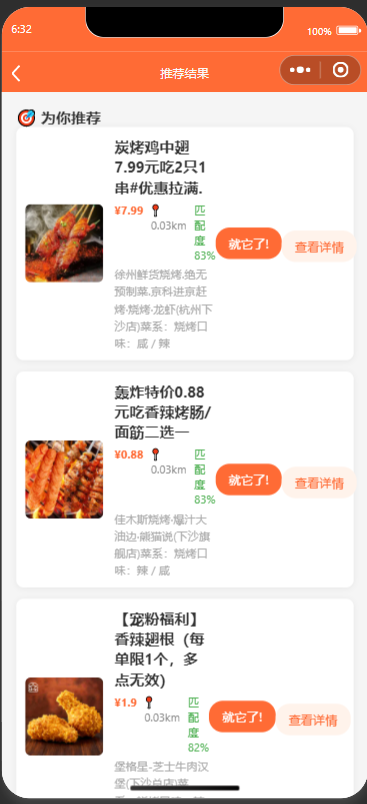
\includegraphics[width=0.75\textwidth,height=0.75\textheight,keepaspectratio]{images/3-4.png}
\caption{推荐结果页界面截图}
\label{fig:3-4}
\end{figure}

\subsection{菜品管理模块实现}

菜品管理模块实现店铺与菜品信息的录入、查询及语义向量生成。后端在菜品录入时同步触发向量化流程：将菜品的名称、菜系、口味标签、描述、食材及城市按固定模板拼接为语义文本，经 sentence-transformers 编码为 768 维向量后回写至数据库。若模型不可用，服务返回 503 状态码并拒绝写入，防止无效向量进入候选池。

\begin{lstlisting}[language=Python, caption={菜品管理模块后端核心实现}]
@router.post("/dishes", response_model=DishOut)
def create_dish(body: DishCreate, user: User = Depends(get_current_user), db: Session = Depends(get_db)):
    dish = Dish(**body.model_dump(exclude_none=True))
    # 同步触发向量化
    shop_name = None
    if dish.shop_id:
        shop = db.query(Shop).filter(Shop.id == dish.shop_id).first()
        shop_name = shop.name if shop else None
    try:
        dish.vector = generate_dish_vector(
            name=dish.name, cuisine=dish.cuisine,
            taste_tags=dish.taste_tags, description=dish.description,
            ingredients=dish.ingredients, city=dish.city,
            latitude=dish.latitude, longitude=dish.longitude,
            shop_name=shop_name,
        )
    except ModelUnavailableError as exc:
        raise HTTPException(status_code=503, detail=str(exc))
    db.add(dish); db.commit(); db.refresh(dish)
    return dish
\end{lstlisting}

前端菜品录入页面向管理员或授权用户，提供店铺信息表单与菜品信息表单。店铺信息包括名称、地址、城市及经纬度；菜品信息包括名称、价格、菜系、口味标签、描述、食材及营养信息。提交成功后前端展示提示并返回个人中心。

\FloatBarrier
\begin{figure}[H]
\centering
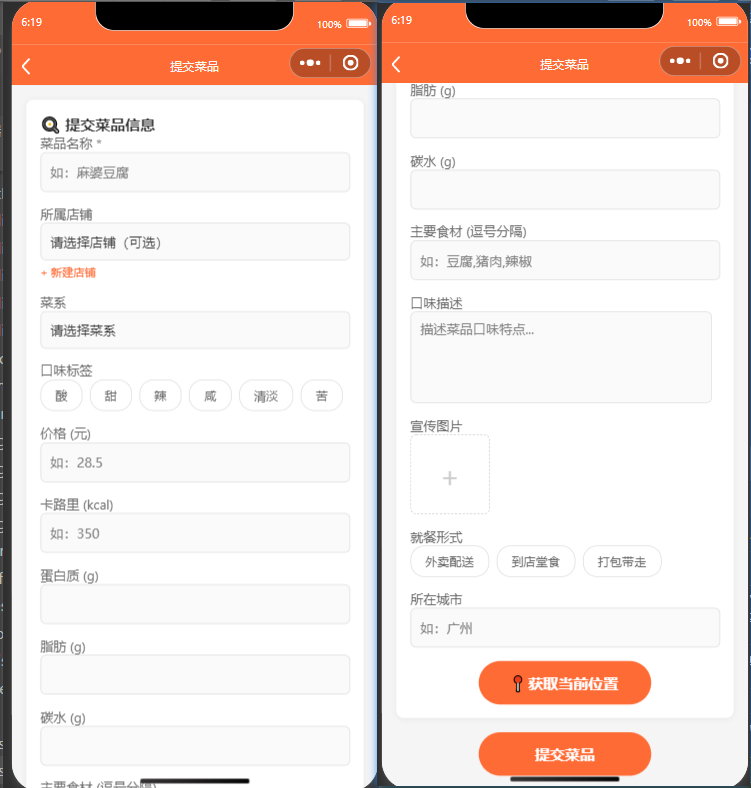
\includegraphics[width=0.8\textwidth]{images/3-5.png}
\caption{菜品录入页界面截图}
\label{fig:3-5}
\end{figure}

\subsection{历史记录与数据闭环模块实现}

历史记录与数据闭环模块实现用户选择行为的持久化存储与全链路交互日志记录。后端历史查询接口按时间倒序返回用户过往选择，支持关联查询菜品详情与问答快照。日志记录接口在推荐生成、用户点击与选择确认三个关键节点写入结构化数据，同一批次通过 UUID 关联曝光、确认与负样本记录。

\begin{lstlisting}[language=Python, caption={历史记录与日志模块后端核心实现}]
@router.get("/", response_model=List[HistoryRecordOut])
def get_history(skip: int = 0, limit: int = 20,
    user: User = Depends(get_current_user), db: Session = Depends(get_db)):
    records = (
        db.query(HistoryRecord)
        .options(joinedload(HistoryRecord.dish))
        .filter(HistoryRecord.user_id == user.id)
        .order_by(HistoryRecord.dining_time.desc())
        .offset(skip).limit(limit).all()
    )
    result = []
    for r in records:
        out = HistoryRecordOut.model_validate(r)
        if r.dish:
            out.dish_name = r.dish.name
            out.price = float(r.dish.price) if r.dish.price else None
            out.cuisine = r.dish.cuisine; out.taste_tags = r.dish.taste_tags
            out.image_url = (r.dish.image_urls or [None])[0]
            if r.dish.shop: out.shop_name = r.dish.shop.name
        result.append(out)
    return result
\end{lstlisting}

前端历史记录页按时间倒序展示过往选择，每条记录展示菜品图片、名称、价格、就餐时间及问答场景摘要。用户点击记录可查看详情，或点击"再来一次"基于历史问答快照重新发起推荐。

\begin{figure}[H]
\centering
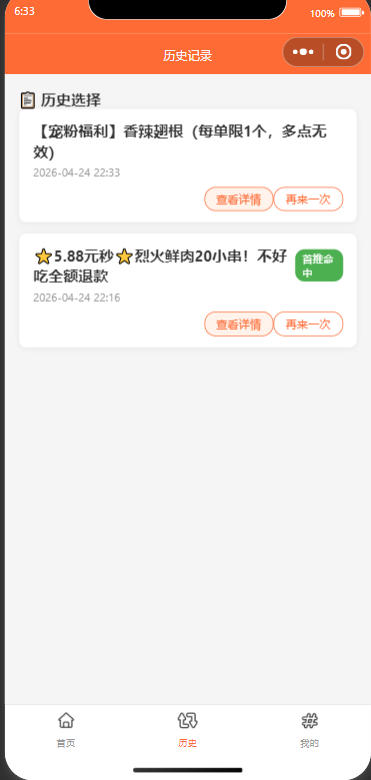
\includegraphics[width=0.8\textwidth,height=0.7\textheight,keepaspectratio]{images/3-6.png}
\caption{历史记录页界面截图}
\label{fig:3-6}
\end{figure}

\FloatBarrier
\section{本章小结}

本章从设计和实现两个角度介绍了系统全貌。概要设计阶段把系统拆成小程序、后端 API、推荐引擎和数据存储四个部分，理清了各自的职责边界。数据库部分设计了七张表，通过外键把用户、画像、店铺、菜品、历史记录和日志关联起来。详细设计阶段逐个梳理了认证、画像、菜品向量化、推荐计算和历史日志五个模块的业务流程，其中推荐引擎是重点，本文给出了硬性过滤的条件定义、向量融合公式和综合得分的计算方式。实现阶段展示了后端各模块的代码组织和前端页面的交互逻辑。以上内容已经通过后续的功能测试验证了可行性。
